\section{Methodology}
\label{sec:method}

To navigate complex, dynamic human environments, a robot must do more than treat sound as a geometric goal. SAVNav processes social acoustic events as persistent social boundaries. The architecture has three modules: multi-modal perception, SAVMap, and the SAVNav policy.

\subsection{Problem Formulation and Notation}
\label{subsec:problem_formulation}

We formalize the SAVNav task in a continuous 3D environment populated by dynamic human agents. Let $\mathcal{E}$ denote the environment, which contains a set of static obstacles $\mathcal{O}_{static}$ (e.g., walls and furniture) and a set of dynamic human agents $\mathcal{H} = \{H_1, H_2, \dots, H_N\}$.

The robot's state at time step $t$ is denoted by its pose $\mathbf{p}_{robot}^{(t)} \in \mathrm{SE}(3)$. The robot is tasked with fulfilling a natural language query $q$ by navigating to a specific acoustic target $A_{target}$, such as a ringing doorbell or a call for help. We define successful task completion as reaching a state where $\|\mathbf{p}_{robot}^{(t)} - \mathbf{p}_{target}\| \le d_{success}$, where $\mathbf{p}_{target}$ is the ground-truth location of $A_{target}$ and $d_{success}$ is the distance threshold.

Simultaneously, the human agents $H_i \in \mathcal{H}$ may engage in social acoustic events $A_i$ (e.g., footsteps or conversations) that propagate through $\mathcal{E}$. The robot does not have access to the ground-truth states of $\mathcal{H}$; it must infer their presence, locations, and social boundaries from egocentric sensory observations. We define an observation $O^{(t)} = (I^{(t)}, D^{(t)}, W^{(t)})$, comprising an RGB image $I^{(t)}$, a depth map $D^{(t)}$, and a $2.55\,\mathrm{s}$ first-order Ambisonics (FOA) audio waveform $W^{(t)}$ ending at time $t$.

The objective is to compute a sequence of velocity commands $\mathbf{v}^{(t)}$ that minimizes the time to reach $A_{target}$ while avoiding physical collisions with $\mathcal{O}_{static} \cup \mathcal{H}$ and minimizing intrusions into the unobservable social boundaries of $\mathcal{H}$. A summary of the key mathematical notations used throughout this section is provided in Table~\ref{tab:notation}.

\begin{table}[ht]
    \centering
    \caption{Summary of key notations}
    \label{tab:notation}
    \resizebox{\linewidth}{!}{
        \begin{tabular}{cl}
            \toprule
            \textbf{Symbol}                              & \textbf{Definition}                                                         \\
            \midrule
            $\mathbf{p}_{vis}, \sigma_{vis}$             & 3D position and spatial uncertainty of a visually detected entity           \\
            $(\theta_{azi}, \theta_{ele}), \sigma_{ang}$ & Egocentric acoustic DOA and its angular uncertainty                         \\
            $\mathbf{d}_{world}$                         & Acoustic DOA vector transformed into the world frame                        \\
            $S_{anchor}^{(t)}(E_i)$                      & Anchoring confidence score linking an acoustic event to visual entity $E_i$ \\
            $\mathbf{p}_{inferred}$                      & Topological node position for NLOS social acoustic events                   \\
            $\mathbf{v}_{infer}$                         & Inferred velocity vector of an NLOS DP                                      \\
            $C_{soc}(\mathbf{x})$                        & Continuous social cost field evaluated at spatial location $\mathbf{x}$     \\
            $\mathcal{M}_{belief}(\mathbf{x})$           & Target spatial belief map for resolving acoustic ambiguity                  \\
            $U(p_i)$                                     & Information-theoretic utility of sampling candidate viewpoint $p_i$         \\
            $S(\mathbf{x})$                              & Speed field used in the Fast Marching Method (FMM) planner                  \\
            \bottomrule
        \end{tabular}
    }
\end{table}

\begin{figure*}[t]
    \centering
    % Insert the system architecture diagram here.
    % The figure should illustrate:
    % 1. Perception (YOLO + embed-ACCDOA) extracting entities and DOA.
    % 2. SAVMap (sparse audio-visual anchoring and topology-aware acoustic anticipation converting audio to Cost Fields).
    % 3. SAVNav Planner (State Machine toggling between Active Search and FMM Planning).
    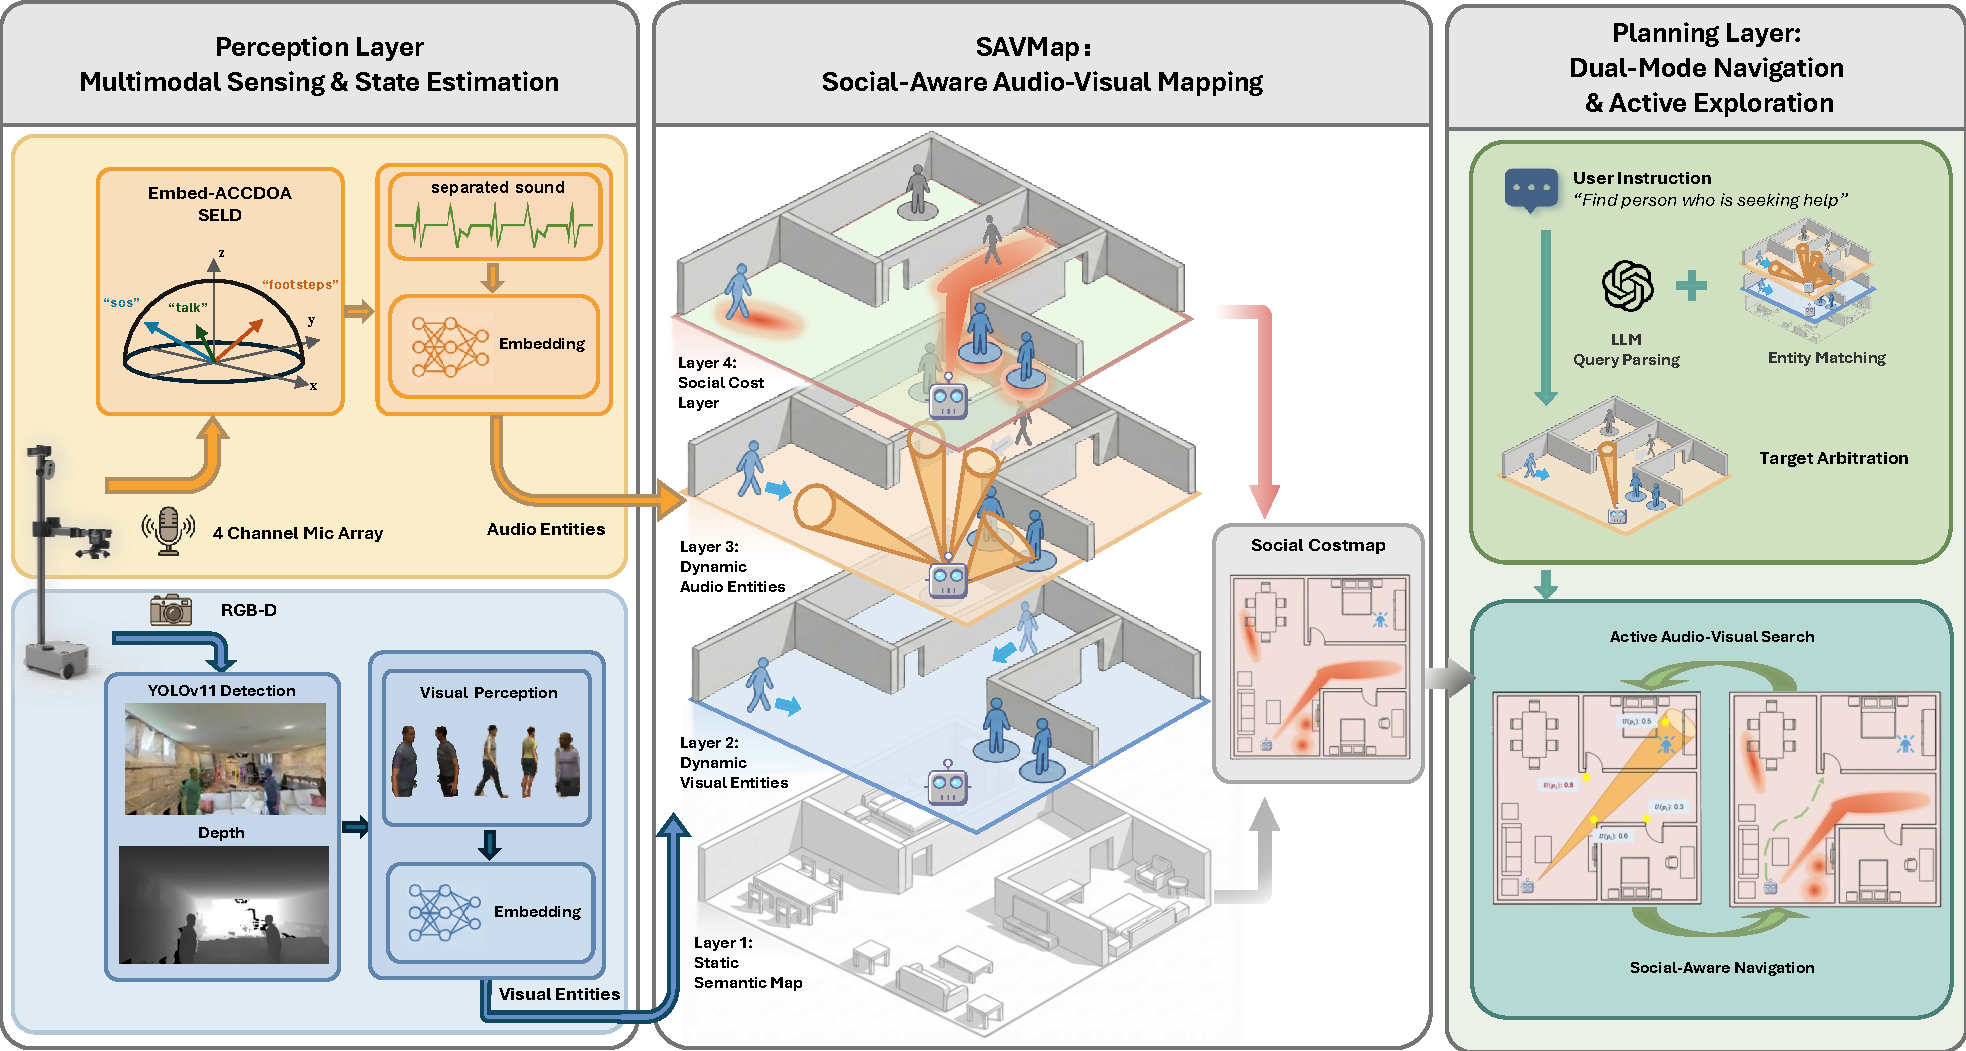
\includegraphics[width=1.00\linewidth]{figures/method.pdf}
    \caption{System architecture of SAVNav. Multi-modal sensory inputs (RGB-D and Ambisonics audio) are processed to extract visual entities and acoustic DOA. These are fused into SAVMap, a spatio-temporal representation that uses sparse audio-visual anchoring and topology-aware acoustic anticipation to map social acoustic events into persistent, anisotropic social cost fields. The SAVNav policy then yields to inferred boundaries and disambiguates uncertain acoustic targets through information-theoretic search.}
    \label{fig:system_arch}
\end{figure*}

\subsection{Multi-Modal Perception}
\label{subsec:perception}

The perception layer extracts spatial and semantic attributes from raw sensory streams and transforms them into object-centric representations.

\subsubsection{Visual Perception}
Operating at $20\,\mathrm{Hz}$, the visual module processes RGB-D inputs using YOLO26~\cite{YOLO26KeyArchitectural2026} for human detection. For each detected bounding box, we extract the 3D position $\mathbf{p}_{vis} \in \mathbb{R}^3$ via depth projection. To quantify measurement uncertainty caused by distance and occlusion, we assign a spatial uncertainty $\sigma_{vis} = k_d z^2 + k_{occ} (1 - \gamma_{mask})$, where $z$ is depth and $\gamma_{mask}$ is the segmentation mask ratio. Semantic features are extracted using ImageBind~\cite{ImageBindOneEmbedding2023}.

\subsubsection{Acoustic Perception}
The acoustic module processes FOA audio streams. Given the transient nature of social acoustic events, we use a sliding-window strategy and feed $2.55\,\mathrm{s}$ audio clips into the embed-ACCDOA model~\cite{OpenvocabularySoundEvent2025} every $0.5\,\mathrm{s}$. This yields the direction-of-arrival (DOA), denoted as angles $(\theta_{azi}, \theta_{ele})$ in the ego frame, together with the associated contrastive language-audio pretraining (CLAP) semantic embedding~\cite{CLAPLearningAudio2023}. The ego-centric DOA is then transformed into a world-frame directional vector $\mathbf{d}_{world} \in \mathbb{R}^3$ by querying the robot's pose at the event timestamp. To account for localization noise, we assign an angular uncertainty $\sigma_{ang}$ that is scaled by the model's confidence output.

\subsection{Acoustic-to-Spatial Social Mapping (SAVMap)}
\label{subsec:savmap}

Traditional social navigation relies on instantaneous, LOS detections. SAVMap addresses this by maintaining a spatio-temporal memory that anchors noisy acoustic vectors to physical geometry and generates dynamic social cost fields.

\subsubsection{Sparse Audio-Visual Anchoring}
Acoustic DOA estimates are inherently noisy and lack depth information. To stably map audio events such as footsteps or chatting to physical entities, we introduce a sparse audio-visual anchoring state machine.

For each incoming acoustic event $A$, we evaluate its spatial and semantic consistency against all tracked visual entities within the DOA cone, defined by $\sigma_{ang}$. The anchoring confidence $S_{anchor}$ for an entity $E_i$ is recursively updated:
\begin{equation}
    S_{anchor}^{(t)}(E_i) = S_{anchor}^{(t-1)}(E_i) + \alpha \cdot sim \cdot \exp\left(-\frac{\theta_{dev}^2}{2\sigma_{ang}^2}\right)
\end{equation}
where $sim$ is the cosine similarity between the acoustic and visual embeddings, $\theta_{dev}$ is the angular deviation from the DOA ray, and $\alpha$ is the update step size. Entities outside the cone experience exponential decay. A hysteresis mechanism suppresses erratic anchoring caused by single-frame SELD errors and requires $S_{anchor} > \tau_{anchor}$ to anchor and $S_{anchor} < \tau_{deanchor}$ to release. Once anchored, the audio event inherits the 3D position and uncertainty of the visual entity.

\subsubsection{Topology-Aware Acoustic Anticipation}
The main challenge in socially-aware navigation is reacting to NLOS risks. When an acoustic event such as footsteps from an NLOS DP or chatting from an NLOS SCG remains unanchored to any visual entity, SAVMap uses topology-aware acoustic anticipation.

Instead of treating the sound as only an ambiguous directional cone, the system casts a ray along $\mathbf{d}_{world}$. Upon intersecting a physical wall, it queries the static semantic map to identify the nearest topological node, such as a corner or a doorway, denoted by $\mathbf{p}_{inferred}$. The subsequent representation depends on the event's semantic classification: if the sound indicates dynamic pedestrians, we inject an inferred velocity vector $\mathbf{v}_{infer}$ pointing from the topological node toward the robot:
\begin{equation}
    \mathbf{v}_{infer} = v_{walk} \cdot \frac{\mathbf{p}_{robot} - \mathbf{p}_{inferred}}{\|\mathbf{p}_{robot} - \mathbf{p}_{inferred}\|}
\end{equation}
where $v_{walk}$ represents a standard human walking speed, predicting that an NLOS DP is likely approaching from the adjacent corridor. Conversely, if the sound indicates a stationary group, we place the inferred SCG at $\mathbf{p}_{inferred}$ without a velocity vector. This maps semantic acoustic cues to their corresponding spatial interactions.

\subsubsection{Anisotropic Social Cost Fields}
To influence robot behavior, SAVMap translates anchored and inferred entities into a continuous social cost field $C_{soc}(\mathbf{x}) \in [0, 1]$. We use dynamic Gaussian fields to represent different social semantics:

\begin{enumerate}
    \item \textit{Stationary Interactions (Chatting):} Modeled as isotropic Gaussians centered at $\mathbf{p}_{entity}$ for anchored entities, or $\mathbf{p}_{inferred}$ for an NLOS SCG, so the robot keeps a polite radius around social groups.
    \item \textit{Approaching Pedestrians (Footsteps):} Modeled as asymmetric anisotropic Gaussians. The spatial variance is elongated along the forward velocity vector, which is $\mathbf{v}$ for anchored entities or $\mathbf{v}_{infer}$ for inferred NLOS DPs:
          \begin{equation}
              C_{soc, dp}(\mathbf{x}) = A \cdot \exp \left( - \left( \frac{d_{long}^2}{2\sigma_{long}^2} + \frac{d_{lat}^2}{2\sigma_{base}^2} \right) \right)
          \end{equation}
          where $d_{long}$ and $d_{lat}$ are the longitudinal and lateral distances to the velocity vector. The forward spread $\sigma_{long}$ scales linearly with speed and prevents the robot from crossing the pedestrian's anticipated path.
\end{enumerate}

\subsection{Proactive Socially-Aware Navigation Policy (SAVNav policy)}
\label{subsec:savnav}

The SAVNav policy translates the spatial constraints of SAVMap into safe, target-driven motion. The planner yields to social boundaries and disambiguates target locations when acoustic evidence is uncertain.

\subsubsection{Active Sensory Exploration}
If the acoustic target, such as a call for help, is detected but remains unanchored due to occlusion or reverberation, the robot enters an active exploration state. We maintain a target spatial belief map $\mathcal{M}_{belief}(\mathbf{x})$, which receives positive updates within the acoustic DOA cone and negative updates in visually cleared empty space.

To resolve target ambiguity, the robot samples candidate viewpoints $\mathcal{P} = \{p_1, \dots, p_N\}$ near topological nodes and within the DOA cone. The optimal viewpoint $p^*$ is selected by maximizing an information-theoretic utility function:
\begin{equation}
    U(p_i) = \sum_{\mathbf{c} \in \mathcal{S}(p_i)} \mathcal{M}_{belief}(\mathbf{c}) \cdot \gamma(\|\mathbf{c} - p_i\|) - \beta \cdot \frac{L(\mathbf{p}_{robot}, p_i)}{v_{avg}}
\end{equation}
where $\mathcal{S}(p_i)$ is the visible frustum area from viewpoint $p_i$, $\gamma(\cdot)$ penalizes excessive observation distance, $L(\cdot)$ computes the geodesic path length, and $\beta$ balances exploration gain against travel time. This makes the robot move to observe ambiguous acoustic regions instead of following noisy audio vectors directly.

\subsubsection{Socially-Compliant Precision Navigation}
Once the acoustic target is anchored, or a clear viewpoint $p^*$ is selected, the system generates smooth, collision-free trajectories. We formulate this as wave propagation in a heterogeneous medium and solve the Eikonal equation using the Fast Marching Method (FMM)~\cite{FastMarchingMethods1999}. The speed field $S(\mathbf{x})$ is defined inversely proportional to the social cost:
\begin{equation}
    S(\mathbf{x}) = S_{max} \cdot \left(1 - w_{soc} \cdot C_{soc}(\mathbf{x})\right) + S_{min}
\end{equation}
The inclusion of the base speed $S_{min}$ ensures that, while the robot prefers to route around social boundaries such as SCGs or the extended risk fields of NLOS DPs, it will not become stuck in dense crowds. Gradient descent on the resulting arrival-time field produces socially compliant paths that curve around both LOS humans and anticipated NLOS DPs.
